\section{Calcolo di derivate}


\subsection{Derivate delle funzioni elementari}

\subsubsection{Asintotici notevoli}
I prossimi teoremi torneranno utili al calcolo delle derivate delle funzioni elementari e corrispondono ai cosiddetti limiti notevoli:
\begin{teor}
	\label{deriv:nepero}
	\[
		\ln(1+\varepsilon)\sim\varepsilon \qquad \varepsilon\to 0
	\]
\end{teor}
\begin{proof}
	Per cambio di variabili:
	\[
		\lim_{\varepsilon\to\infty} \left(1+\frac{1}{\varepsilon}\right)^\varepsilon=e\Rightarrow\lim_{\varepsilon\to0} (1+\varepsilon)^{1/\varepsilon}=e
	\]
	Tramite uguaglianza di logaritmi:
	\begin{gather*}
		\lim_{\varepsilon\to0} \ln [(1+\varepsilon)^{\frac{1}{\varepsilon}}]=\ln e\\
		\lim_{\varepsilon\to0} \frac{1}{\varepsilon}\ln(1+\varepsilon)=1\\
		\ln(1+\varepsilon)\sim\varepsilon
	\end{gather*}
\end{proof}

\begin{teor}
	\label{deriv:nepero2}
	\[
		e^\varepsilon-1\sim\varepsilon\qquad\varepsilon\to0
	\]
\end{teor}
\begin{proof}
	\[
		\lim_{\varepsilon\to0} \frac{e^\varepsilon-1}{\varepsilon} =
	\]
	Cambiando variabile, con $t=e^\varepsilon-1$ che tende a $0$ e quindi $\varepsilon=\ln(1+t)$:
	\[
		= \lim_{t\to0} \frac{t}{\ln(1+t)}
	\]
	Per il teorema precedente il denominatore è asintotico a $t$, quindi il limite vale $1$.
\end{proof}

\begin{teor}
	\label{deriv:nepero3}
	\[
		(1+\varepsilon)^\alpha-1\sim\alpha\varepsilon\qquad\varepsilon\to0
	\]
\end{teor}
\begin{proof}
	Applicando il teorema \ref{deriv:nepero} con $\varepsilon=(1+t)^\alpha-1$, e quindi $t=(\varepsilon+1)^{\frac{1}{\alpha}}-1$, che tende a $0$ per $\varepsilon$ tendente a $0$:
	\[
		1=\lim_{\varepsilon\to0}\frac{\ln (1+\varepsilon)}{\varepsilon}=\lim_{t\to0}\frac{\ln(1+[(1+t)^\alpha-1])}{(1+t)^\alpha-1}=\lim_{t\to0}\frac{\alpha\ln(1+t)}{(1+t)^\alpha-1}
	\]
	Applicando nuovamente il teorema \ref{deriv:nepero}, questa volta alla variabile $t$, otteniamo che $\ln(1+t)\sim t$, quindi, poiché l'asintotico non influisce sul risultato dei limiti:
	\[
		\lim_{t\to0}\frac{\alpha\ln(1+t)}{(1+t)^\alpha-1}=\lim_{t\to0}\frac{\alpha t}{(1+t)^\alpha-1}
	\]
	Poiché questo limite è uguale a $1$, è dimostrato che $\alpha t\sim (1+t)^\alpha-1$.
\end{proof}

I prossimi due teoremi riguardano asintotici relativi a funzioni goniometriche:
\begin{teor}
	\label{deriv:sin}
	\[
		\sin h\sim h\qquad h\to0
	\]
\end{teor}
\begin{proof}
	Si noti che nel limite da dimostrare
	\[
		\lim_{h\to0} \frac{\sin h}{h}=1
	\]
	le funzioni al numeratore e al denominatore sono entrambe dispari, per cui il loro quoziente è pari\footnote{Infatti, se si sostituisce ad $h$ il suo opposto $-h$ la frazione risultante sarà uguale a quella originaria: $\frac{\sin -h}{-h}=\frac{-\sin h}{-h}=\frac{\sin h}{h}$}. Da questo si può dedurre che l'esistenza del limite destro
	\[
		\lim_{h\to0^+} \frac{\sin h}{h}=1
	\]
	implica l'esistenza e l'uguaglianza del limite sinistro ($h\to0^-$), e quindi del limite di partenza ($h\to0$). Si può dunque per la dimostrazione ipotizzare che $h$ sia positivo, inoltre poiché tende a $0$ lo si può porre minore di qualunque soglia positiva, per esempio $0<h<\frac{\pi}{2}$.

	Si faccia riferimento alla figura \ref{fig:dersin}, in cui sulla circonferenza goniometrica unitaria $h$ è l'angolo in radianti, nonché misura dell'arco di circonferenza $BC$ (per la definizione di radiante).
	\begin{figure}[ht]
		\centering
		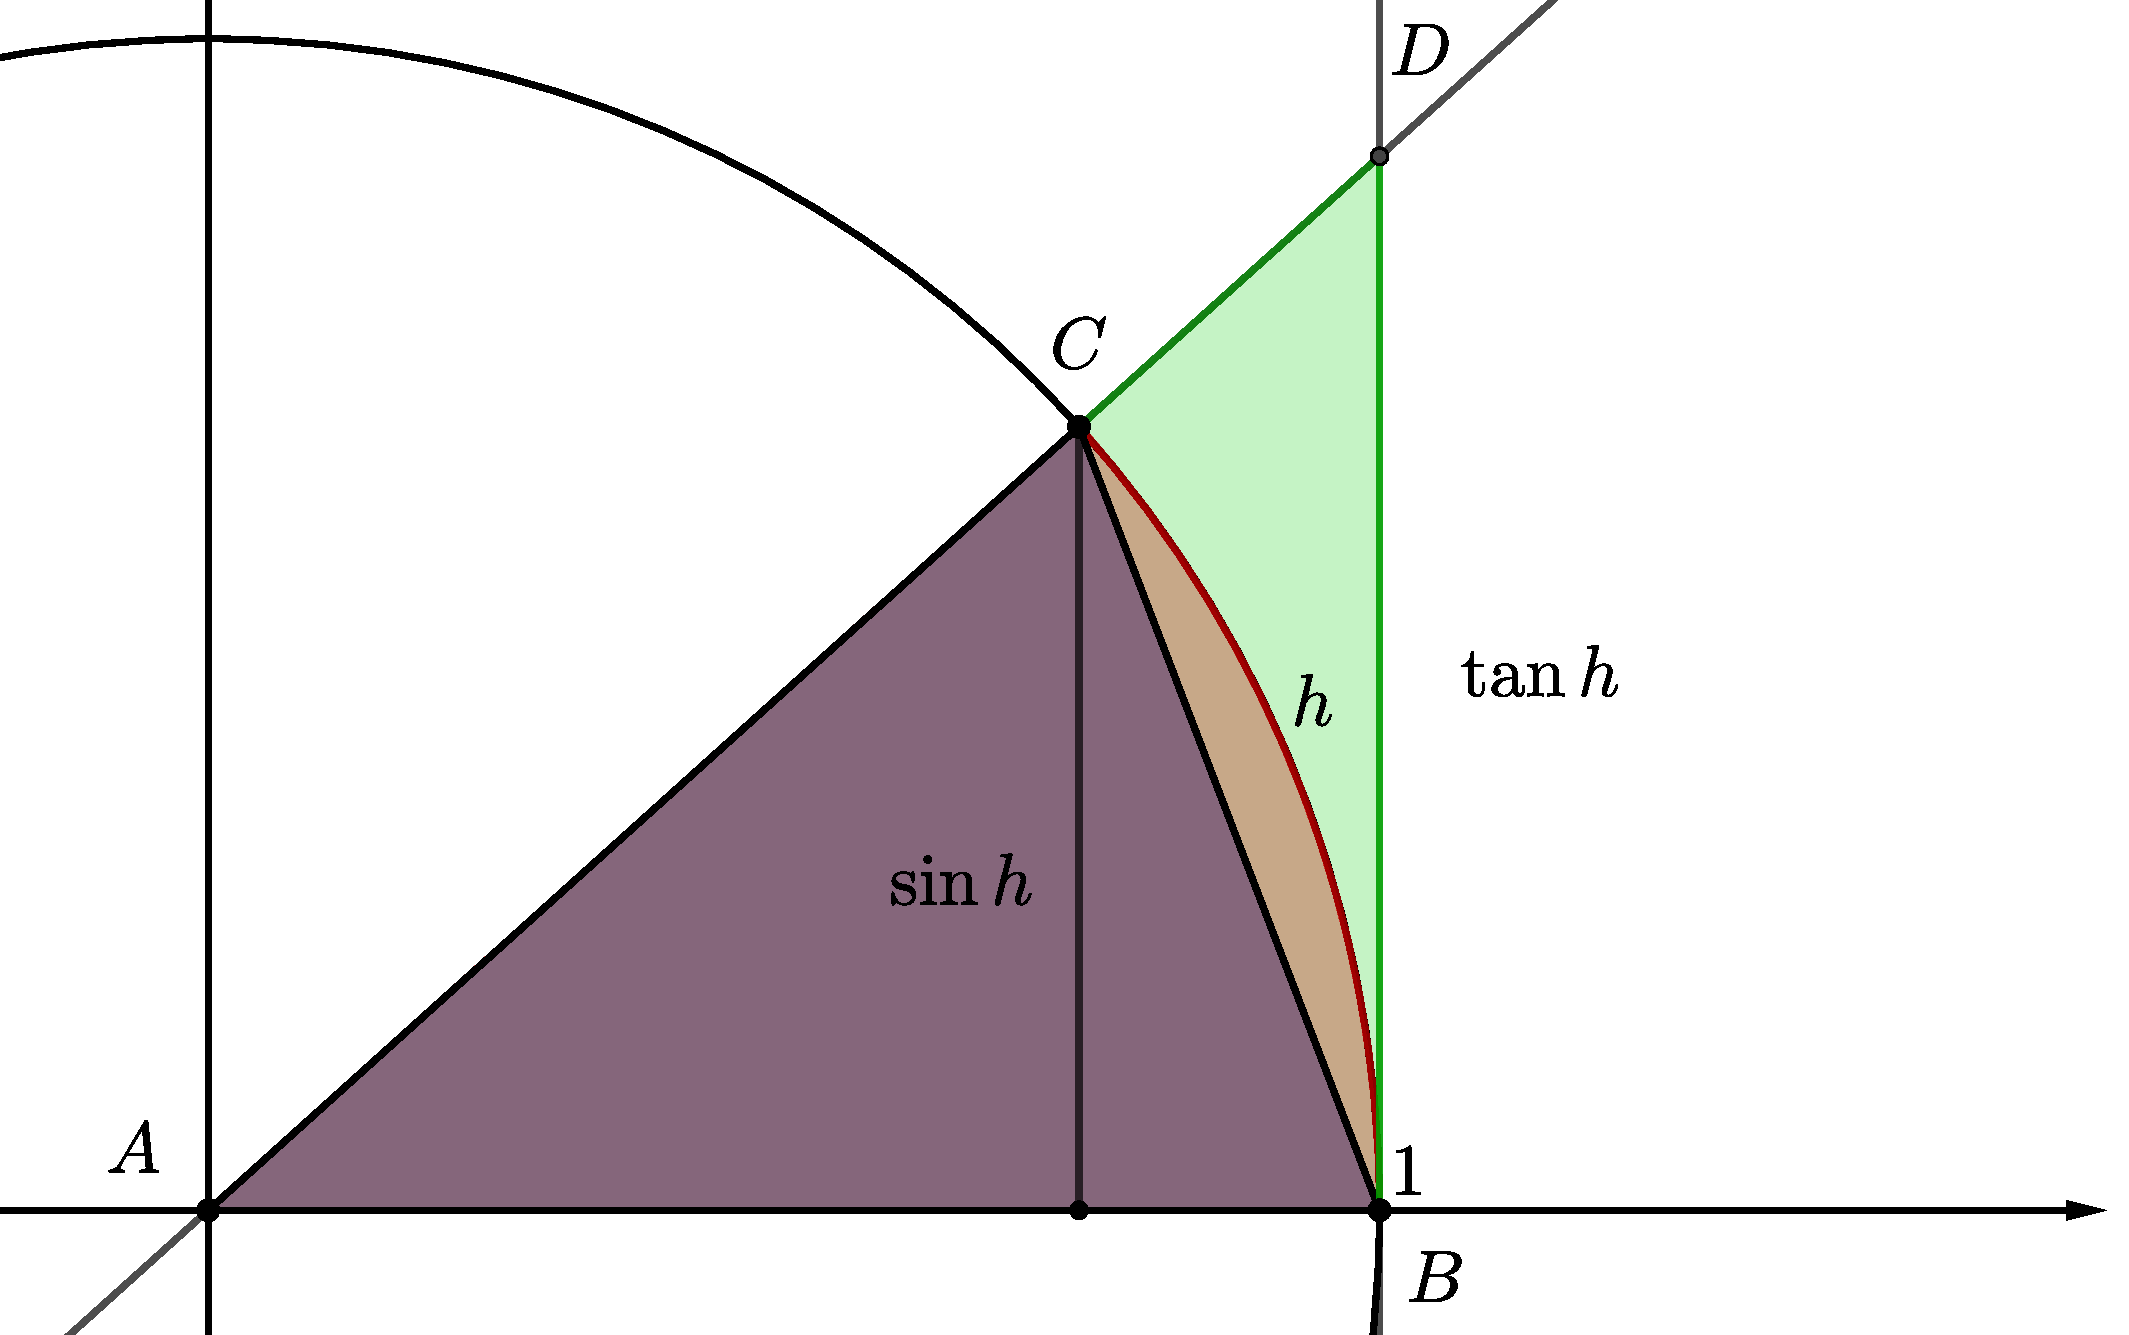
\includegraphics[width=0.7\textwidth]{grafici/sin_notevole}
		\caption{Le tre aree della disuguaglianza per la dimostrazione del limite notevole del seno.}
		\label{fig:dersin}
	\end{figure}
	Si nota che le aree del triangolo $ABC$, del settore circolare di angolo $h$, diciamo $S$ e del triangolo $ABD$ sono legate dalla relazione:
	\begin{equation}
		\label{dersin:dis}
		A_{ABC}<A_S<A_{ABD}
	\end{equation}
	La prima area vale $\frac{\overline{AB}*\sin h}{2}$, cioè, poiché $\overline{AB}=1$ per costruzione, $\frac{\sin h}{2}$. La terza area vale per lo stesso motivo $\frac{\tan h}{2}$. La seconda area invece è quella del settore circolare di angolo $h$, da cui per proporzionalità diretta con l'angolo giro vale:
	\[
		\frac{A_{\text{cerchio}}}{2\pi}=\frac{A_S}{h}
	\]
	Poiché l'area del cerchio unitario è $\pi\cdot 1^2=\pi$, $A_S=\frac{h}{2}$. La disuguaglianza \ref{dersin:dis} è quindi uguale a
	\[
		\frac{\sin h}{2}<\frac{h}{2}<\frac{\tan h}{2}
	\]
	Si moltiplica ora per $2$ e si divide per $\sin h$, che si sa essere positivo poiché $0<h<\frac{\pi}{2}$, per cui la disequazione mantiene il verso $<$:
	\begin{gather*}
		\frac{\sin h}{\sin h}<\frac{h}{\sin h}<\frac{\tan h}{\sin h}\\
		1<\frac{h}{\sin h}<\frac{1}{\cos h}
	\end{gather*}
	Poiché per $h\to0$ $\frac{1}{\cos h}$ tende a $1$, si applica il teorema del confronto (\vref{teor:confronto}) e si dimostra così che
	\[
		\lim_{h\to0^+} \frac{h}{\sin h}=\lim_{h\to0} \frac{\sin h}{h}=1
	\]
\end{proof}

\begin{teor}
	\label{deriv:cos}
	\[
		1-\cos h\sim \frac{h^2}{2}\qquad h\to0
	\]
\end{teor}
\begin{proof}
	In generale:
	\[
		1=\sin^2 h+\cos^2 h
	\]
	Per $h$ vicino a $0$ il coseno è positivo, quindi:
	\[
		\cos h=+\sqrt{1-\sin^2 h}
	\]
	Per il teorema precedente e per $h\to0$, $\sin h\sim h$, che in termini di $o$ piccolo equivale a $\sin h=h+o(h)$. Quindi l'uguaglianza equivale\footnote{si ricorda che nello sviluppo del quadrato $[h+o(h)]^2=h^2+2h*o(h)+[o(h)]^2$, il quadrato $[o(h)]^2$ è uguale a $o(h^2)$, mentre il doppio prodotto viene assorbito da $o(h^2)$} a
	\begin{equation}
		\label{eq:coseq}
		\cos h=\sqrt{1-[h+o(h)]^2}=\sqrt{1-h^2+o(h^2)}
	\end{equation}
	Traducendo il teorema \ref{deriv:nepero3} in termini di $o$ piccolo ($\varepsilon\to0$):
	\[
		(1+\varepsilon)^\alpha-1\sim\alpha\varepsilon\Rightarrow (1+\varepsilon)^\alpha-1=\alpha\varepsilon+o(\varepsilon)\Rightarrow (1+\varepsilon)^\alpha=1+\alpha\varepsilon+o(\varepsilon)
	\]
	applicato alla \ref{eq:coseq}, usando $\alpha=\frac{1}{2}$ e $\varepsilon=-h^2+o(h^2)$:
	\[
		\sqrt{1-h^2+o(h^2)}=1+\frac{1}{2}[-h^2+o(h^2)]+o[-h^2+o(h^2)]=
	\]
	Poiché $-h^2+o(h^2)\sim -h^2$:
	\[
		=1-\frac{1}{2}h^2+o(h^2)+o(h^2)=1-\frac{h^2}{2}+o(h^2)
	\]
	Riportandosi all'equazione iniziale:
	\[
		\cos h=1-\frac{h^2}{2}+o(h^2)\Rightarrow 1-\cos h=\frac{h^2}{2}+o(h^2)
	\]
	che tradotto in asintotico equivale a
	\[
		1-\cos h\sim\frac{h^2}{2}
	\]
\end{proof}

\subsubsection{Derivate elementari}
Calcoliamo ora, avvalendoci di tali teoremi, le derivate delle funzioni elementari:
\begin{itemize}
	\item $f(x)=\ln x$. Per $h\to0$:
	      \[
		      \frac{\ln (x_0+h)-\ln x_0}{h}=\frac{1}{h}\ln\left(\frac{x_0+h}{x_0}\right)=\frac{1}{h}\ln\left(1+\frac{h}{x_0}\right)
	      \]
	      Applicando il teorema \ref{deriv:nepero} con $\varepsilon=\frac{h}{x_0}$ (che tende a $0$):
	      \[
		      \frac{1}{h}\ln\left(1+\frac{h}{x_0}\right)\sim\frac{1}{h}\cdot \frac{h}{x_0}=\frac{1}{x_0}
	      \]
	\item $f(x)=\log_q x$. Considerato che, per cambio di base, $\log_q x=\log_q e\cdot \ln x_0$, il procedimento precedente può essere ripetuto con la costante moltiplicativa $\log_q e$, per cui la derivata sarà
	      \[
		      \frac{\log_q e}{x_0}
	      \]
	\item $f(x)=e^x$. Per $h\to0$:
	      \[
		      \frac{e^{x_0+h}-e^{x_0}}{h}=\frac{e^{x_0}e^h-e^{x_0}}{h}=e^{x_0}\frac{e^h-1}{h}
	      \]
	      Per il teorema \ref{deriv:nepero2}, con $\varepsilon=h\to0$:
	      \[
		      e^{x_0}\frac{e^h-1}{h}\sim e^{x_0}\frac{h}{h}=e^{x_0}
	      \]
	\item $f(x)=x^n$ con $n\in\N\setminus 0$. Per sviluppare la potenza della funzione incrementata si utilizza il binomio di Newton. Per $h\to0$:
	      \[
		      \frac{(x_0+h)^n-x_0^n}{h}=\frac{1}{h}\left[\left(\sum_{k=0}^n \binom{n}{k}h^k x_0^{n-k}\right)-x_0^n\right]
	      \]
	      Come si può intuire dallo sviluppo del teorema \ref{derivo}, sono i termini lineari in $h$ (cioè in cui $h$ è di primo grado) quelli a essere fondamentali per il calcolo della derivata; in particolare, tutti i termini che contengono $h$ elevato a esponenti maggiori o uguali a $2$ possono essere riassunti nel termine\footnote{con la semplificazione in $o(h)$ avviene una perdita di informazione, la cui però non ci è utile alla dimostrazione.} $o(h)$. La sommatoria può quindi essere semplificata in
	      \[
		      \frac{1}{h}\cdot \left[\left(x_0^n+\binom{n}{1}h x_0^{n-1}+o(h)\right)-x_0^n\right]=
	      \]
	      Sviluppando il coefficiente e ricordando che per definizione $\frac{o(h)}{h}=o(1)$:
	      \[
		      =\frac{x_0^n+nhx_0^{n-1}+o(h)-x_0^n}{h}=nx^{n-1}+o(1)\to nx^{n-1}
	      \]
	\item $f(x)=x^\alpha$, con $\alpha\in\R\land x\geq0$. Per $h\to0$:
	      \[
		      \frac{(x_0+h)^\alpha-x_0^\alpha}{h}=x_0^\alpha\cdot \frac{(1+\frac{h}{x_0})^\alpha-1}{h}
	      \]
	      Applicando il teorema \ref{deriv:nepero3}, con $\varepsilon=\frac{h}{x}\to0$:
	      \[
		      x_0^\alpha\cdot \frac{(1+\frac{h}{x_0})^\alpha-1}{h}\sim x^\alpha\cdot \frac{\alpha\frac{h}{x_0}}{h}\to\alpha x^{\alpha-1}
	      \]
	\item $f(x)=\sin x$. Utilizzando le formule goniometriche di addizione, per $h\to0$:
	      \begin{gather*}
		      \frac{\sin(x_0+h)-\sin x_0}{h}=\frac{\sin x_0\cos h+\cos x_0\sin h-\sin x_0}{h}=\\
		      \sin x_0 \cdot \frac{\cos h -1}{h}+\cos x_0 \cdot \frac{\sin h}{h}=
	      \end{gather*}
	      Applicando i teoremi \ref{deriv:sin} e \ref{deriv:cos}:
	      \[
		      =\sin x_0 \cdot \frac{-\frac{h^2}{2}}{h}+\cos x_0 \cdot \frac{h}{h}\to \cos x_0
	      \]
	\item $f(x)=\cos(x)$ Utilizzando le formule goniometriche di addizione, per $h\to0$:
	      \begin{gather*}
		      \frac{\cos(x_0+h)-\cos x_0}{h}=\frac{\cos x_0\cos h-\sin x_0\sin h-\cos x_0}{h}=\\
		      \cos x_0 \cdot \frac{\cos h -1}{h}-\sin x_0 \cdot \frac{\sin h}{h}=
	      \end{gather*}
	      Come nel caso precedente, si applicano i teoremi \ref{deriv:sin} e \ref{deriv:cos}:
	      \[
		      =\cos x_0 \cdot \frac{-\frac{h^2}{2}}{h}-\sin x_0 \cdot \frac{h}{h}\to-\sin x_0
	      \]
\end{itemize}


\subsection{Derivate non elementari}
Per calcolare la derivata di una funzione non elementare, è necessario ricavare metodi che permettano di calcolare la derivata di un'operazione tra funzioni (addizione, moltiplicazione, etc.). Questi metodi sono racchiusi in alcuni bteoremi. Le dimostrazioni di questi utilizzano per lo più lo sviluppo della funzione incrementata di cui al teorema \vref{derivo}.

\subsubsection{Derivata della somma}
\begin{prop}[Derivata della somma]
	Date due funzioni $f$ e $g$ derivabili in $x_0$:
	\[
		(f+g)'(x_0)=f'(x_0)+g'(x_0)
	\]
\end{prop}
\begin{proof}
	La somma incrementata delle due funzioni è, per lo sviluppo di cui al teorema \ref{derivo} (per $h\to0$):
	\begin{gather*}
		(f+g)(x_0+h)=f(x_0+h)+g(x_0+h)=\\
		(f(x_0)+f'(x_0)h+o(h))+(g(x_0)+g'(x_0)h+o(h))=\\
		=f(x_0)+g(x_0)+(f'(x_0)+g'(x_0))h+o(h)=\\
		(f+g)(x_0)+(f+g)'(x_0)h+o(h)
	\end{gather*}
	L'esistenza e la qualità dello sviluppo dimostra che la derivata è quella espressa dalla tesi.
\end{proof}
\begin{prop}[Derivata del prodotto]
	\label{der:prod}
	Date due funzioni $f$ e $g$ derivabili in $x_0$:
	\[
		(fg)'(x_0)=f(x_0)g'(x_0)+f'(x_0)g(x_0)
	\]
	La somma incrementata delle due funzioni è, per lo sviluppo di cui al teorema \ref{derivo} (per $h\to0$):
\end{prop}
\begin{proof}
	% TODO: aggiungere spiegazione o(h)
	\begin{gather*}
		(fg)(x_0+h)=f(x_0+h)g(x_0+h)=\\
		[f(x_0)+f'(x_0)h+o(h)][g(x_0)+g'(x_0)h+o(h)]=\\
		=f(x_0)g(x_0)+[f(x_0)g'(x_0)+f'(x_0)g(x_0)]h+o(h)
	\end{gather*}
\end{proof}

\begin{prop}
	% TODO: verificare ipotesi
	\label{der:reci}
	Data una funzione $f$ derivabile in $x_0$ tale che $f(x_0)\neq0$, allora $\frac{1}{f}$ è derivabile in $x_0$ e la sua derivata è uguale a:
	\[
		\left(\frac{1}{f}\right)'(x_0)=-\frac{f'(x_0)}{f^2(x_0)}
	\]
\end{prop}
\begin{proof}
	\begin{gather*}
		\left(\frac{1}{f}\right)(x_0+h)=\frac{1}{f(x_0+h)}=\frac{1}{f(x_0)+f'(x_0)h+o(h)}=\\
		\frac{1}{f(x_0)}\left(1+\frac{f'(x_0)}{f(x_0)}h+o(h)\right)^{-1}=
	\end{gather*}
	Si può applicare ora il limite notevole \ref{deriv:nepero3}, poiché $-\left(\frac{f'(x_0)}{f(x_0)}h+o(h)\right)$ è una quantità infinitesima:
	\[
		=\frac{1}{f(x_0)}\left[1-\left(\frac{f'(x_0)}{f(x_0)}h+o(h)\right)+o\left(-\left(\frac{f'(x_0)}{f(x_0)}h+o(h)\right)\right)\right]=
	\]
	L'argomento di $o$ è perlomeno $O(h)$, per cui l'intero termine $o(O(h))$ è uguale\footnote{Si veda il terzo punto della proprietà \ref{prop:landaugp}} a $o(h)$:
	\begin{gather*}
		=\frac{1}{f(x_0)}\left[1-\frac{f'(x_0)}{f(x_0)}h+o(h)+o(O(h))\right]=\frac{1}{f(x_0)}-\frac{f'(x_0)}{f^2(x_0)}h+o(h)
	\end{gather*}
\end{proof}

\begin{prop}
	Per $g(x_0)\neq0$:
	\[
		\left(\frac{f}{g}\right)'(x_0)=\frac{f'(x_0)g(x_0)-f(x_0)g'(x_0)}{g^2(x_0)}
	\]
\end{prop}
\begin{proof}
	Il quoziente $\frac{f}{g}$ non è altro che il prodotto di $f$ per il reciproco di $g$, quindi, per il teorema \ref{der:prod}:
	\[
		\left(\frac{f}{g}\right)'(x_0)=f'(x_0)\frac{1}{g(x_0)}+f(x_0)\left(\frac{1}{g(x_0)}\right)'=
	\]
	Per il teorema \ref{der:reci}:
	\[
		=f'(x_0)\frac{1}{g(x_0)}+f(x_0)\left(-\frac{g'(x_0)}{g^2(x_0)}\right)=\frac{f'(x_0)g(x_0)-f(x_0)g'(x_0)}{g^2(x_0)}
	\]
\end{proof}

\begin{prop}[Derivata di funzione composta]
	\label{der:comp}
	\[
		\begin{cases}
			g \text{ derivabile in $x_0$} \\
			f \text{ derivabile in $g(x_0)$}
		\end{cases}\Rightarrow
		\begin{cases}
			(f\circ g)(x_0)\text{ derivabile in $x_0$} \\
			(f\circ g)'(x_0)=f'(g(x_0))g'(x_0)
		\end{cases}
	\]
\end{prop}
\begin{proof}
	Per $h\to0$
	\begin{equation*}
		(f\circ g)(x_0+h)=f(g(x_0+h))=f(g(x_0)+\underbrace{g'(x_0)h+o(h)}_{k})=
	\end{equation*}
	La quantità $k=g'(x_0)h+o(h)$ tende a $0$ per $h\to0$. L'espressione può essere dunque vista come la funzione incrementata $f(g(x_0)+k)$. Sfruttando l'ipotesi della deribabilità di $f$ in $g(x_0)$, si può scrivere lo sviluppo:
	\begin{gather*}
		f(g(x_0))+f'(g(x_0))[g'(x_0)h+o(h)]+o(g'(x_0)h+o(h)) = \\
		(f\circ g)(x_0)+f'(g(x_0))g'(x_0)h+\underbrace{f'(g(x_0))o(h)+o(g'(x_0)h+o(h))}_{o(h)} = \\
		(f\circ g)(x_0)+f'(g(x_0))g'(x_0)h+o(h)
	\end{gather*}
\end{proof}

\begin{prop}[Derivata dell'inversa]
	Per $f'(x_0)\neq0$:
	\[
		Df^{-1}(y)=\frac{1}{Df(f^{-1}(y))}
	\]
\end{prop}
\begin{proof}
	Poiché $f^{-1}(y)$ è l'inversa di $f(y)$, si verifica che $f(f^{-1}(y))=y$. Utilizzando il teorema \ref{der:comp} per le funzioni composte:
	\[
		D(f(f^{-1}(y)))=Df(f^{-1}(y))\cdot Df^{-1}(y)
	\]
	Questa derivata è uguale a $1$ in quanto la funzione è uguale a $y$ per ogni $y$. Questo ci permette di ricavare la derivata della funzione inversa, ovvero il secondo fattore:
	\[
		Df^{-1}(y)=\frac{1}{Df(f^{-1}(y))}
	\]
\end{proof}

\begin{examp}
	La derivata dell'arcotangente, definita come la funzione inversa della tangente per l'intervallo $-\frac{\pi}{2},\frac{\pi}{2}$, si può calcolare applicando il teorema appena dimostrato:
	\[
		D\arctan y=\frac{1}{\tan'(\arctan y)}=\cos^2(\arctan y)
	\]
	Chiamiamo $\theta=\arctan y$. Dividendo il risultato per $1=\sin^2\theta+\cos^2\theta$:
	\[
		\frac{\cos^2\theta}{\sin^2\theta+\cos^2\theta}=\frac{1}{\frac{\sin^2\theta+\cos^2\theta}{\cos^2\theta}}=\frac{1}{\tan^2\theta+1}
	\]
	Poiché $\tan\theta=\tan(\arctan y)=y$:
	\[
		D\arctan y=\frac{1}{y^2+1}
	\]
\end{examp}
